\documentclass[10pt,a4paper]{article}

% --- Layout: tight margins to fit a dense 3-page report ---
\usepackage[margin=1.7cm]{geometry}
\usepackage{amsmath,amssymb}
\usepackage{graphicx}
\usepackage{booktabs}
\usepackage{array}
\usepackage[hidelinks]{hyperref}
\usepackage{caption}
\captionsetup{font=small,labelfont=bf}
\usepackage{titlesec}
\titlespacing*{\section}{0pt}{7pt}{3pt}
\titlespacing*{\subsection}{0pt}{5pt}{2pt}
\setlength{\parskip}{1.5pt}
\setlength{\parindent}{0pt}

% figures are stored next to this file so the report is self-contained
\graphicspath{{figs/}}

\newcommand{\ppar}{\mathrm{pp\text{-}AR}}

\title{\vspace{-1.2cm}\textbf{Recurrent Reasoning Networks for the\\Maximum Independent Set Problem}}
\author{Malik Mardan}
\date{June 8, 2026}

\begin{document}
\maketitle
\vspace{-0.7cm}

\noindent\small This project adapts the Tiny Recursive Model (TRM) of
Jolicoeur-Martineau et al., \emph{Less is More: Recursive Reasoning with Tiny
Networks} (arXiv:2510.04871), from grid puzzles to graph problems. The idea of
TRM is that a very small network, applied many times in a recurrent loop, can
solve hard reasoning tasks that usually call for much larger models. We test
whether that holds for the Maximum Independent Set problem.
Code: \url{https://github.com/73gon/trm-mis}.
\normalsize

%==========================================================================
\section{Approach}

\paragraph{Problem.}
Given an undirected graph $G=(V,E)$, the Maximum Independent Set (MIS) problem
asks for the largest set $S\subseteq V$ in which no two nodes share an edge. MIS
is NP-hard. We frame it as per-node classification: the network outputs a
probability $p_v\in[0,1]$ that node $v$ belongs to an optimal set, and a
deterministic decoder turns these probabilities into a valid independent set.

\paragraph{Architecture.}
The model (\texttt{GraphTransformerTRM}, about $1.55$\,M parameters) combines a
graph-transformer backbone with the recurrent reasoning loop of TRM:
\begin{itemize}\itemsep1pt
  \item \textbf{Inputs.} Each node carries $12$ local structural features
    (degree and normalised degree, clustering coefficient, neighbour-degree
    statistics, and $k$-core number) plus a $16$-dimensional positional encoding.
    These are embedded and concatenated into a $256$-dimensional vector.
  \item \textbf{GPS layers} ($2$ layers, hidden width $256$, $4$ attention
    heads). Every layer runs a local GIN message-passing branch and a global
    self-attention branch in parallel, so a node sees both its neighbourhood and
    the whole graph.
  \item \textbf{Recurrent reasoning.} A latent state $z$ and an output state $y$
    are refined by $H{=}2$ outer cycles of $L{=}6$ inner updates, giving $12$
    reasoning steps in total. Only the final step backpropagates; the earlier
    ones run without gradients. This lets the small network improve its answer
    by repeating computation instead of adding parameters, which is the central
    claim of TRM.
\end{itemize}

\paragraph{Training.}
The model is trained with full supervision. The loss adds a class-weighted binary
cross-entropy on the node labels to a soft feasibility penalty that punishes
giving high probability to both endpoints of an edge:
\[
\mathcal{L}=\mathrm{BCE}_{w}(\sigma(z),y)
   \;+\;\lambda\,\tfrac{1}{2|E|}\!\!\sum_{(u,v)\in E}\! p_u p_v ,
   \qquad \lambda=2 .
\]
Labels come in two flavours. For the small graphs we compute \emph{multi-solution}
targets: Gurobi enumerates up to $16$ strictly optimal independent sets per graph,
and the target $y_v$ is the fraction of those optima that contain node $v$. Such a
target is calibrated, so its own cross-entropy is strictly positive (about $0.19$
at $n{=}50$). For the large benchmarks we use a single near-optimal labelling from
the KaMIS solver together with a positive-class weight $w$ ($w{=}1$ for the small
runs, $w{=}2$ for SATLIB, $w{=}5$ for the dense ER graphs). Optimisation uses AdamW
(weight decay $0.05$), a OneCycle learning-rate schedule (peak $3\times10^{-4}$,
$10\%$ warm-up, cosine decay), \texttt{bf16} precision, and dropout $0.15$, with
early stopping on the held-out test loss.

\paragraph{What the numbers mean.}
\begin{itemize}\itemsep0.5pt
  \item \textbf{Iteration.} One gradient update on one mini-batch of graphs; ``$29$k
    iterations'' means $29{,}000$ updates. We evaluate every $500$ iterations and
    keep the best checkpoint, so runs stop at different counts.
  \item \textbf{Approximation ratio ($\ppar$).} The main quality metric. We decode
    the probabilities greedily (take nodes by probability, skip any neighbour of a
    chosen node) and report $|S_{\text{ours}}|/|S^\star|$; $1.0$ is optimal.
  \item \textbf{Feasibility.} The share of decoded solutions that are valid
    independent sets. Greedy decoding can never pick two adjacent nodes, so it is
    $1.0$ by construction; the difficulty is reaching the optimum, not staying valid.
  \item \textbf{BCE.} Cross-entropy between the predicted probability and the
    training label. It measures calibration against one labelling, which is not the
    same as the quality of the final set (see below).
  \item \textbf{Confusion matrix.} Per node, whether predicted MIS membership
    matches the ground truth, split into true/false positives and negatives.
\end{itemize}

%==========================================================================
\section{Experiments}

We run two studies. The first is a controlled scaling study on
Erd\H{o}s--R\'enyi (ER) graphs of fixed average degree $7.35$ at sizes
$n\in\{50,100,200,300\}$, each with a held-out test split and exact Gurobi labels.
The second uses two larger benchmarks from the DIFUSCO suite: SATLIB (SAT formulas
turned into conflict graphs, around $1400$ nodes) and ER-700-800 (dense ER graphs
of $700$ to $800$ nodes, average degree about $112$), both labelled by KaMIS.

\subsection{Scaling over problem size}

On all four small sizes the model learns cleanly (Fig.~\ref{fig:small}). The test
BCE drops from its random-init value near $0.73$ to between $0.23$ and $0.32$,
while $\ppar$ climbs from about $0.886$ at initialisation to at least $0.98$. Larger
graphs reach their best checkpoint in fewer iterations because each graph carries
more signal, but they also start to overfit sooner since their training pools are
smaller (Table~\ref{tab:main}). The model generalises rather than memorises: train
and test graphs use disjoint random seeds.

\begin{figure}[h]
  \centering
  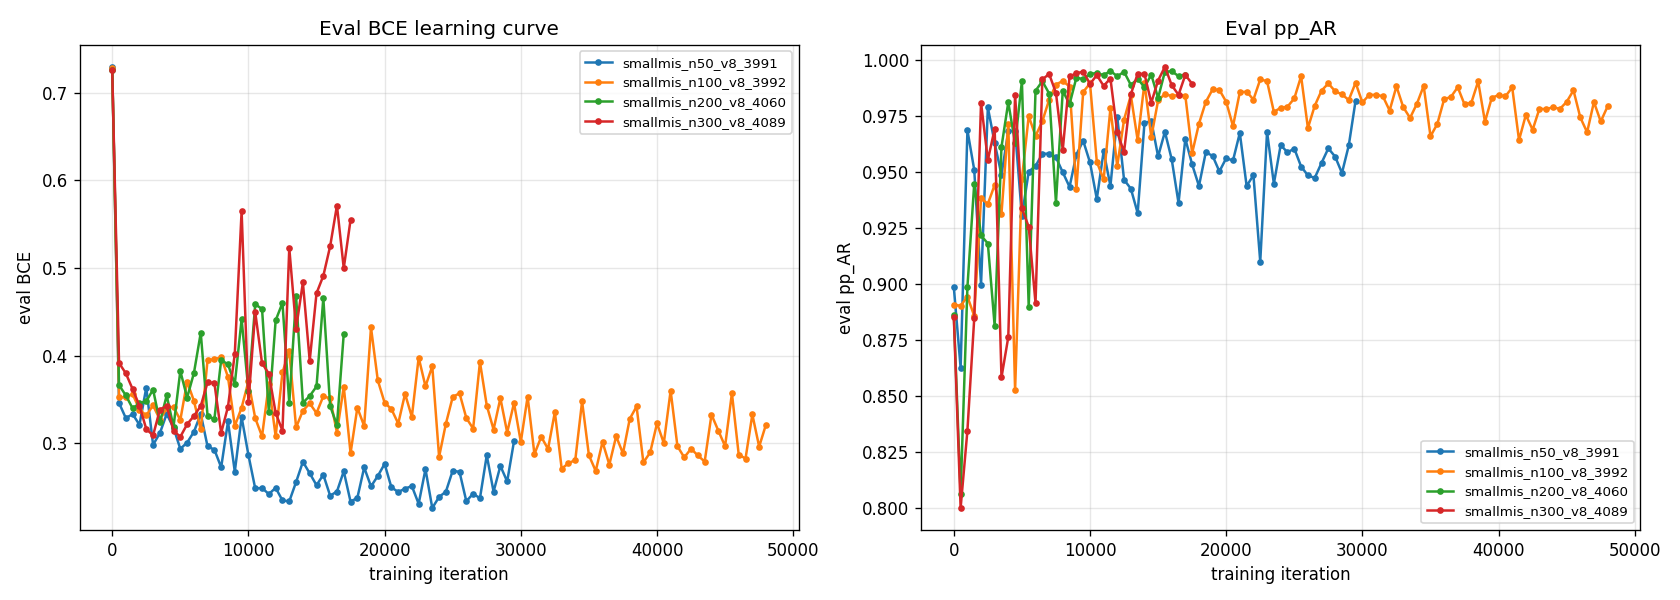
\includegraphics[width=0.66\linewidth]{small_mis_curves.png}
  \caption{Held-out learning curves for the four small ER sizes. Left: test BCE
  (lower is better). Right: approximation ratio $\ppar$ (higher is better).}
  \label{fig:small}
\end{figure}

\begin{table}[h]
\centering
\small
\caption{Main results. The top block is the small-ER scaling study; the bottom
block is the two large benchmarks. $q$ is the average MIS fraction $|S^\star|/n$.
``best BCE'' is the lowest test BCE over the run and ``best $\ppar$'' the highest
test ratio; the two can occur at different checkpoints. Feasibility is $1.00$
everywhere thanks to greedy decoding.}
\label{tab:main}
\begin{tabular}{lrrrrrrr}
\toprule
Dataset & nodes & train graphs & $q$ & best BCE & best $\ppar$ & feas. & iter @ best $\ppar$\\
\midrule
ER $d{=}7.35$ & 50  & 50{,}000 & 0.32 & 0.226 & \textbf{0.982} & 1.00 & 29.5k \\
ER $d{=}7.35$ & 100 & 50{,}000 & 0.34 & 0.268 & \textbf{0.993} & 1.00 & 25.5k \\
ER $d{=}7.35$ & 200 & 12{,}000 & 0.36 & 0.319 & \textbf{0.995} & 1.00 & 11.5k \\
ER $d{=}7.35$ & 300 & \phantom{0}3{,}000 & 0.36 & 0.307 & \textbf{0.997} & 1.00 & 15.5k \\
\midrule
SATLIB        & $\sim$1400 & 9{,}000 & 0.33 & 0.713 & \textbf{0.998} & 1.00 & 150k \\
ER-700-800    & 700--800   & 25{,}000 & 0.06 & n/a   & \textbf{0.903} & 1.00 & 325k \\
\bottomrule
\end{tabular}
\end{table}

\subsection{Why a high BCE can still give a high approximation ratio}

A striking pattern in Table~\ref{tab:main} is that SATLIB reaches the best
approximation ratio of the whole study ($\ppar=0.998$) while its BCE stays around
$0.7$ to $0.8$, far above the small ER runs that sit near $0.25$. The two metrics
measure different things. BCE asks whether each node probability matches one fixed
labelling. The benchmark graphs have many different optimal sets, but KaMIS returns
only one of them, so a node that belongs to some other optimum is labelled $0$ even
though the model sensibly gives it a moderate probability. That mismatch, together
with the positive-class weight, keeps BCE high. The approximation ratio, by
contrast, depends only on the \emph{order} of the probabilities that the greedy
decoder reads off: as long as good MIS nodes rank above the nodes that conflict
with them, the decoded set is near optimal regardless of absolute calibration. The
small ER runs avoid the mismatch because their multi-solution targets are
calibrated, so they reach both a low BCE and a high ratio. In short, BCE tracks
probability calibration against one labelling, $\ppar$ tracks set quality, and only
$\ppar$ reflects the objective we actually care about.

\subsection{Confusion matrices}

Table~\ref{tab:cm} gives the node-level confusion matrix at each best-$\ppar$
checkpoint, as a percentage of all nodes. The small ER models are balanced, with
roughly equal false positives and false negatives and about $90\%$ node accuracy.
The benchmarks behave differently: both over-predict membership (large false-positive
share), yet the greedy decoder still recovers near-optimal sets, which is the same
decoupling discussed above. The dense ER case is the extreme: only $6\%$ of nodes
are in the MIS, the classifier floods the graph with false positives, and node
accuracy looks fine ($73\%$) only because most nodes are correctly rejected.

\begin{table}[h]
\centering
\small
\caption{Node-level confusion matrices at the best-$\ppar$ checkpoint
(\% of all nodes). TP/FP/FN/TN sum to $100$; accuracy is $\text{TP}+\text{TN}$.}
\label{tab:cm}
\begin{tabular}{lrrrrr}
\toprule
Dataset & TP & FP & FN & TN & accuracy \\
\midrule
ER $n{=}50$    & 27.4 & 4.9  & 5.0 & 62.7 & 90.1 \\
ER $n{=}100$   & 28.6 & 6.1  & 5.6 & 59.8 & 88.4 \\
ER $n{=}200$   & 29.9 & 7.2  & 5.9 & 57.0 & 86.9 \\
ER $n{=}300$   & 30.6 & 6.8  & 5.8 & 56.8 & 87.4 \\
\midrule
SATLIB         & 25.6 & 20.6 & 7.7 & 46.1 & 71.7 \\
ER-700-800     & 3.4  & 24.7 & 2.6 & 69.3 & 72.7 \\
\bottomrule
\end{tabular}
\end{table}

\subsection{Scaling up, and where it stopped working}

The benchmark runs used a $9000$-graph training pool. On SATLIB this succeeded and
gave the best result of the study, but the run also shows a clear failure mode of
prolonged training (Fig.~\ref{fig:satlib}). The approximation ratio peaks near
$0.998$ around iteration $150$k and then slowly falls back to $0.95$, while the BCE
climbs from $0.7$ to $1.8$. The model keeps fitting the single KaMIS labelling more
aggressively, which hurts both calibration and, eventually, the decoded sets. Early
stopping on the test score is therefore essential at this scale.

\begin{figure}[h]
  \centering
  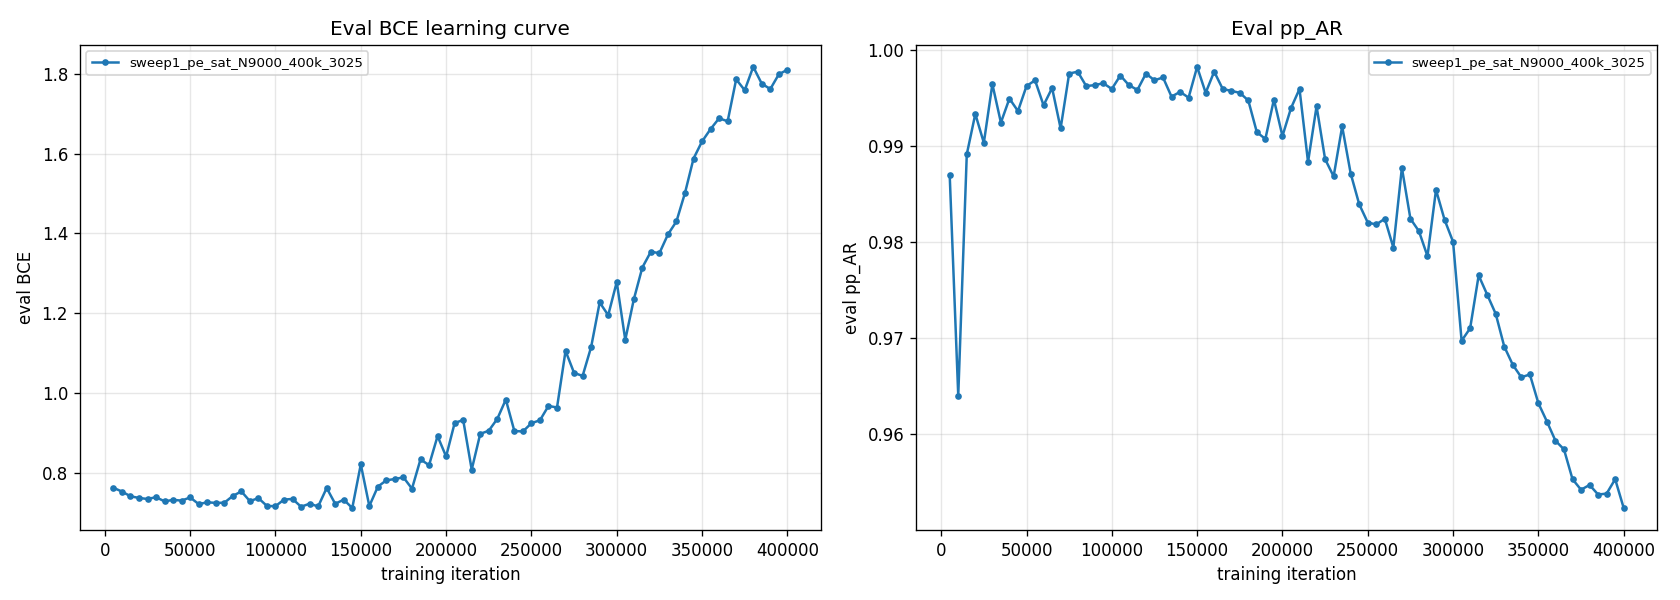
\includegraphics[width=0.66\linewidth]{satlib_n9000.png}
  \caption{SATLIB with a $9000$-graph pool. The ratio peaks near iteration $150$k
  and then degrades as the BCE rises, a clear overfitting signature.}
  \label{fig:satlib}
\end{figure}

The same $9000$-graph setup did not even start on the dense ER-700-800
distribution: both attempts ran out of GPU memory on a $31.4$\,GB card inside the
GIN message-passing step, before a single evaluation. The cause is the edge count,
not the number of graphs. A dense ER graph of $750$ nodes has roughly $40$ times as
many edges per node as a SATLIB conflict graph, so a batch of them produces a far
larger message-passing tensor. The best completed result on this distribution comes
from a smaller in-memory pool ($25{,}000$ graphs in smaller batches), which reaches
$\ppar=0.903$, well above a degree-heuristic baseline of $0.60$ but clearly the
hardest case we tried.

%==========================================================================
\section{Key insights}

\begin{enumerate}\itemsep2pt
  \item \textbf{The tiny recurrent network does learn MIS.} Every small-ER size
    reaches $\ppar$ between $0.98$ and $0.997$ on held-out graphs with a single
    $1.55$\,M model unrolled for $12$ steps, which supports the TRM premise that
    repeated computation can stand in for scale.
  \item \textbf{Set quality and node loss are different objectives.} A model can
    have a poor BCE (SATLIB at $0.7$ to $0.8$, dense ER far worse) and still decode
    near-optimal sets, because the greedy decoder only needs the right ranking.
    Choosing or stopping a run on BCE alone would be misleading; the approximation
    ratio is the metric to watch.
  \item \textbf{Density is the real difficulty axis, not size.} The largest sparse
    graphs (SATLIB, around $1400$ nodes) were easier than smaller but much denser
    ER graphs. Both quality and trainability, including the out-of-memory failure,
    track edge count and the shrinking MIS fraction $q$ rather than node count.
  \item \textbf{Feasibility is free, optimality is the work.} Greedy decoding keeps
    feasibility at $1.00$ everywhere, so the feasibility loss mainly shapes the
    ranking and all remaining effort goes into closing the gap to the optimum.
  \item \textbf{Long training can hurt.} On the large single-solution benchmark the
    approximation ratio peaked and then declined with more training, so a held-out
    stopping criterion matters as much as the model itself.
\end{enumerate}

\vspace{2pt}
\noindent{\footnotesize\textit{Reproducibility.} All training, data-generation, and
plotting code, the dataset specifications, and the configuration files are in the
repository at \url{https://github.com/73gon/trm-mis}. The figures are regenerated by
the plotting script from the training logs.\par}

\end{document}
